\section{Tính đơn điệu và cực trị của hàm số}
\subsection{Lý thuyết cần nhớ}
\subsubsection{Tính đơn điệu của hàm số}
\begin{enumerate}[\iconMT]
	\item \indam{Định nghĩa:} Cho hàm số $y=f(x)$ xác định trên $K$ ($K$ là khoảng, đoạn hoặc nửa khoảng). 
\begin{minipage}[b]{8cm}
\begin{khung4}{Ghi nhớ 1}
	Hàm số đồng biến trên $K$ nếu
	$$\forall x_1,\,x_2 \in K\colon x_1<x_2 \Rightarrow f(x_1)<f(x_2)$$
	\centerline{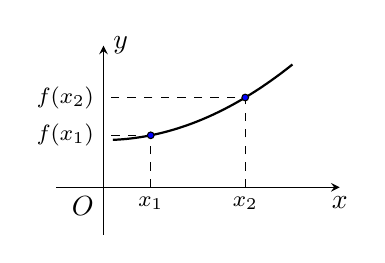
\begin{tikzpicture}[>=stealth,scale=0.6]
		\draw[->] (-1,0)--(0,0)%
		node[below left]{$O$}--(5,0) node[below]{$x$};
		\draw[->] (0,-1) --(0,3) node[right]{$y$};
		\draw [black,thick, domain=0.2:4, samples=100] %
		plot (\x, {0.1*(\x)^2+1});
		\draw [dashed] (1,0)node[below]{\footnotesize$x_1$} --(1,1.1)--(0,1.1)node[left]{\footnotesize$f(x_1)$};
		\draw [dashed] (3,0)node[below]{\footnotesize$x_2$} --(3,1.9)--(0,1.9)node[left]{\footnotesize$f(x_2)$};
		\draw[fill=blue] (1,1.1) circle(2pt);
		\draw[fill=blue] (3,1.9) circle(2pt);
	\end{tikzpicture}}\\
Trên $K$, đồ thị là một "\textbf{đường đi lên}" khi xét từ trái sang phải.
\end{khung4}
\end{minipage}\hspace{0.5cm}
\begin{minipage}[b]{8cm}
\begin{khung4}{Ghi nhớ 2}
		Hàm số nghịch biến trên $K$ nếu
		$$\forall x_1,\,x_2 \in K\colon x_1<x_2 \Rightarrow f(x_1)>f(x_2)$$
		\centerline{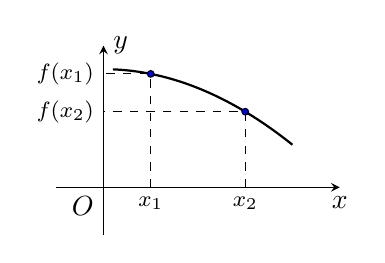
\begin{tikzpicture}[>=stealth,scale=0.6]
			\draw[->] (-1,0)--(0,0)%
			node[below left]{$O$}--(5,0) node[below]{$x$};
			\draw[->] (0,-1) --(0,3) node[right]{$y$};
			\draw [thick, domain=0.2:4, samples=100] %
			plot (\x, {-0.1*(\x)^2+2.5});
			\draw [dashed] (1,0)node[below]{\footnotesize$x_1$} --(1,2.4)--(0,2.4)node[left]{\footnotesize$f(x_1)$};
			\draw [dashed] (3,0)node[below]{\footnotesize$x_2$} --(3,1.6)--(0,1.6)node[left]{\footnotesize$f(x_2)$};
			\draw[fill=blue] (1,2.4) circle(2pt);
			\draw[fill=blue] (3,1.6) circle(2pt);
		\end{tikzpicture}}\\
	Trên $K$, đồ thị là một "\textbf{đường đi xuống}" khi xét từ trái sang phải.
\end{khung4}
\end{minipage}
	\item \indam{Liên hệ giữa đạo hàm và tính đơn điệu:}
	Cho hàm số $y=f(x)$ có đạo hàm trên khoảng $(a;b)$.
	\begin{boxdn}
	\begin{listEX}[1]
		\item [$\bullet$] Nếu $y'\ge 0$, $\forall x \in (a;b)$ và dấu bằng chỉ xảy ra tại hữu hạn điểm thì hàm số $y=f(x)$ đồng biến trên $(a;b)$.
		\item [$\bullet$] Nếu $y'\le 0$, $\forall x \in (a;b)$ và dấu bằng chỉ xảy ra tại hữu hạn điểm thì hàm số  $y=f(x)$ nghịch biến trên $(a;b)$.
	\end{listEX}
	\end{boxdn}
\end{enumerate}
\subsubsection{Cực trị của hàm số}
\begin{enumerate}[\iconMT]
	\item \indam{Định nghĩa:} Cho hàm số $y=f(x)$ xác định và liên tục trên khoảng $(a ; b)$ và điểm $x_0 \in(a ; b)$.
	\begin{boxdn}
	\begin{itemize}
		\item [$\bullet$] Nếu tồn tại số $h>0$ sao cho $f(x)<f\left(x_0\right)$ với mọi $x \in\left(x_0-h ; x_0+h\right) \subset(a ; b)$ và $x \neq x_0$ thì ta nói hàm số $f(x)$ đạt cực đại tại $x_0$.
		\item [$\bullet$] Nếu tồn tại số $h>0$ sao cho $f(x)>f\left(x_0\right)$ với mọi $x \in\left(x_0-h ; x_0+h\right) \subset(a ; b)$ và $x \neq x_0$ thì ta nói hàm số $f(x)$ đạt cực tiểu tại $x_0$.
	\end{itemize}
	\end{boxdn}
	\item \indam{Định lý:} Giả sử hàm số $y=f(x)$ liên tục trên khoảng $(a ; b)$ chứa điểm $x_0$ và có đạo hàm trên các khoảng $\left(a ; x_0\right)$ và $\left(x_0 ; b\right)$. Khi đó:
	\begin{boxdn}
	\begin{itemize}
		\item [$\bullet$] Nếu $f^{\prime}(x)<0$ với mọi $x \in\left(a ; x_0\right)$ và $f^{\prime}(x)>0$ với mọi $x \in\left(x_0 ; b\right)$ thì $x_0$ là một điểm cực tiểu của hàm số $f(x)$.
		\item [$\bullet$] Nếu $f^{\prime}(x)>0$ với mọi $x \in\left(a ; x_0\right)$ và $f^{\prime}(x)<0$ với mọi $x \in\left(x_0 ; b\right)$ thì $x_0$ là một điểm cực đại của hàm số $f(x)$.
	\end{itemize}
	\end{boxdn}
	\item \indam{Các tên gọi:}\\
		\hspace*{2cm}\begin{tikzpicture}[smooth,samples=300,scale=1.15,>=stealth]
			\draw[->,>=stealth] (-2.5,0)--(2.7,0) node[below]{$x$};
			\draw[->,>=stealth] (0,-1.5)--(0,4) node[right]{$y$};
			\draw (0,0) node[above left]{$O$};
			\draw[blue,domain=-2:2,line width = 1.2pt] plot(\x,{(\x)^3-3*(\x)+1})node[right]{$y=f(x)$};
			\draw[fill=black] (1,0) circle(1pt) (1,-1) circle(2pt) (0,-1) circle(1pt) (-1,0) circle(1pt) (-1,3) circle(2pt) (0,3) circle(1pt);
			\draw[dashed] (1,0)node[above]{\small$x_2$}--(1,-1)--(0,-1)node[left]{\small$y_2$} (-1,0)node[below]{\small$x_1$}--(-1,3)--(0,3)node[right]{\small$y_1$};
			
			\draw[-,dotted] (-0.5,3.7)--(4,3.7)node[right]{$(x_1;y_1)$ là điểm cực đại của đồ thị hàm số;}; 
			\draw[->,dotted] (-0.5,3.7)--(-1,3.15);
			\node[right] at (4.5,3.1) {$\bullet$ $x_1$ là điểm cực đại của hàm số;};
			\node[right] at (4.5,2.5) {$\bullet$ $y_1$ là giá trị cực đại của hàm số.};
			
			\draw[-,dotted] (2,-1)--(2,1)--(4,1)node[right]{$(x_2;y_2)$ là điểm cực tiểu của đồ thị hàm số;}; \draw[->,dotted] (2,-1)--(1.15,-1);
			\node[right] at (4.5,0.4) {$\bullet$ $x_2$ là điểm cực tiểu của hàm số;};
			\node[right] at (4.5,-0.2) {$\bullet$ $y_2$ là giá trị cực tiểu của hàm số.};
		\end{tikzpicture}
\end{enumerate}

\subsection{Phân loại và phương pháp giải toán}
\begin{dang}{Bài toán khoảng đơn điệu và cực trị của hàm số cho trước}
	\begin{listEX}[1]
		\item [\ding{172}] Tìm tập xác định $\mathscr{D}$ của hàm số $y=f(x)$ .
		\item [\ding{173}] Tính đạo hàm $f'(x)$. Tìm các điểm $x_i \,(i = 1, 2, ..., n)$ thuộc $\mathscr{D}$ mà tại đó $f'(x)=0$ hoặc $f'(x)$ không xác định.
		\item [\ding{174}] Sắp xếp các điểm $x_i$ theo thứ tự tăng dần, xét dấu $y'$ và lập bảng biến thiên. Từ đây, nêu các khoảng đồng biến, nghịch biến và các điểm cực trị.
	\end{listEX}
\end{dang}

\boxmini{BÀI TẬP TỰ LUẬN}

\begin{vd}
	Tìm các khoảng đơn điệu và các điểm cực trị của hàm số sau
	\begin{tasks}(3)
		\task $y = -x^2 + 4x - 3$;
		\task $ y=x^3-3x^2+1$;
		\task $y=x^3+3x^2+3x+2$;
		\task $y=-2x^4+4x^2$;
		\task $y=x^4+4x^3-1$;
		\task $y=-16x^4+x-1$.
	\end{tasks}
	\loigiai{
	\begin{enumEX}[a)]{1}
		\item Tập xác định: $\mathscr{D} = \mathbb{R}$.\\
		Đạo hàm: $y' = -2x + 4$. Cho $y' = 0 \Leftrightarrow -2x + 4 = 0 \Leftrightarrow x = 2$.\\
		Bảng biến thiên:\begin{center}
			
\begin{tikzpicture}
				\tkzTabInit[nocadre=false,espcl=3,lgt=1.5]
				{$x$/0.6,$y'$/0.6,$y$/2.2}
				{$-\infty$,$2$,$+\infty$}
				\tkzTabLine{,+,0,-,}
				\tkzTabVar{-/$-\infty$,+/$1$,-/$-\infty$}
			\end{tikzpicture}
		\end{center}
	Hàm số đồng biến trên khoảng $(-\infty; 2)$ và nghịch biến trên khoảng $(2; +\infty)$.\\
	Hàm số đạt cực đại tại $x = 2$, giá trị cực đại $y_{CĐ} = 1$. Hàm số không có cực tiểu.
		\item Ta có: $ y'=3x^2-6x\Rightarrow y'=0\Leftrightarrow \hoac{&x=0\\&x=2.} $\\
		Từ bảng biến thiên suy ra hàm số đồng biến trên khoảng $ (-\infty;0) $ và $ (2;+\infty). $
		\begin{center}
			
\begin{tikzpicture}
				\tkzTabInit[nocadre=false,lgt=1,espcl=3]
				{$x$ /1,$y'$ /1,$y$ /2}
				{$-\infty$,$0$, $2$,$+\infty$}
				\tkzTabLine{,+,$0$,-,$0$,+, }
				\tkzTabVar{-/ $-\infty$,+/$1 $ ,-/$-3$,+/$+\infty$}
			\end{tikzpicture}
		\end{center}
		\item Hàm số đã cho xác định trên $\mathscr{D}=\mathbb{R}$.\\
		Ta có $y'=3x^2+6x+3$. Cho $y'=0 \Leftrightarrow 3x^2+6x+3=0 \Leftrightarrow x=-1$.\\
		Bảng biến thiên
		\begin{center}
			
\begin{tikzpicture}
				\tkzTabInit[lgt=1,espcl=3]
				{$x$/0.7,$y'$/0.7,$y$/2}
				{$-\infty$,$-1$,$+\infty$}
				\tkzTabLine{,+,0,+,}
				\tkzTabVar{-/$-\infty$,R/,+/$+\infty$}
				
			\end{tikzpicture}
		\end{center}
		Vậy hàm số đồng biến trên $\mathbb{R}$.
		\item Tập xác định của hàm số là $ \mathscr{D}=\mathbb{R}$.\\
		Ta có $y'=-8x^3+8x$.
		Cho $y'=0 \Leftrightarrow -8x^3+8x=0 \Leftrightarrow 8x(-x^2+1)=0$\\
		\centerline{$ \Leftrightarrow \left[\begin{aligned}
				&8x=0 \\
				&-x^2+1=0
			\end{aligned}\right. \Leftrightarrow \left[\begin{aligned}
				&x=0 \\
				&x^2=1
			\end{aligned}\right. \Leftrightarrow \left[\begin{aligned}
				&x=0 \\
				&x=\pm 1.
			\end{aligned}\right. $}
		Bảng biến thiên
		\begin{center}
			
\begin{tikzpicture}
				\tkzTabInit[lgt=1,espcl=3]
				{$x$/0.7,$y'$/0.7,$y$/2}
				{$-\infty$,$-1$,$0$,$1$,$+\infty$}
				\tkzTabLine{,+,0,-,0,+,0,-,}
				\tkzTabVar{-/$-\infty$,+/ $2$/,-/$0$,+/$2$,-/$-\infty$}
			\end{tikzpicture}
		\end{center}
		Vậy hàm số đồng biến trên mỗi khoảng $(-\infty;-1)$ và $(0;1)$,\\
		\indent{ } hàm số nghịch biến trên mỗi khoảng $(-1;0)$ và $(1;+\infty)$.
		\item Hàm số đã cho xác định trên $\mathscr{D}=\mathbb{R}$.\\
		Ta có $y'=4x^3+12x^2=0=4x^2(x+3)$.\\
		Cho $y'=0 \Leftrightarrow 4x^2(x+3)=0 \Leftrightarrow \left[\begin{aligned}
			&x=0 \\
			&x=-3.
		\end{aligned}\right.$\\
		Bảng biến thiên
		\begin{center}
			
\begin{tikzpicture}
				\tkzTabInit[lgt=1,espcl=3]
				{$x$/0.7,$y'$/0.7,$y$/2}
				{$-\infty$,$-3$,$0$,$+\infty$}
				\tkzTabLine{,-,0,+,0,+,}
				\tkzTabVar{+/$+\infty$,-/$-28$ /,R,+/$+\infty$}
			\end{tikzpicture}
		\end{center}
		Vậy hàm số nghịch biến trên khoảng $(-\infty;-3)$ và đồng biến trên khoảng $(-3;+\infty)$.
		\item Ta có $y'=-64x^3+1<0\Leftrightarrow x>\dfrac{1}{4}$ nên hàm số nghịch biến trên khoảng $\left(\dfrac{1}{4};+\infty\right)$.
\end{enumEX}}
\end{vd}
\dongcham{47}
\begin{vd}
	Tìm các khoảng đơn điệu và cực trị của các hàm số sau:
	\begin{enumEX}[a)]{3}
		\item $y=\sqrt{9-x^2}$;
		\item $y=\sqrt{x^2-2x}$;
		\item $y=x-3\sqrt[3]{x^2}$.
	\end{enumEX}
\loigiai{
\begin{enumEX}[a)]{1}
	\item Hàm số xác định khi $9 - x^2 \ge 0 \Leftrightarrow -3 \le x \le 3$. 
	Vậy $D = [-3; 3]$.\\
	Ta có: $y' = \dfrac{(9 - x^2)'}{2\sqrt{9 - x^2}} = \dfrac{-2x}{2\sqrt{9 - x^2}} = \dfrac{-x}{\sqrt{9 - x^2}}$.\\
	Cho $y' = 0 \Leftrightarrow -x = 0 \Leftrightarrow x = 0 \in (-3; 3)$.\\
	Bảng biến thiên: 
	\begin{center}
		
\begin{tikzpicture}
			\tkzTabInit[nocadre=false,lgt=1.2,espcl=2.5]
			{$x$ /0.6, $y'$ /0.6, $y$ /2}
			{$-3$, $0$, $3$}
			\tkzTabLine{d, +, 0, -, d}
			\tkzTabVar{-/$0$, +/$3$, -/$0$}
		\end{tikzpicture}
	\end{center}
	Dựa vào bảng biến thiên, ta có:
	\begin{itemize}
		\item Hàm số \textbf{đồng biến} trên khoảng $(-3; 0)$.
		\item Hàm số \textbf{nghịch biến} trên khoảng $(0; 3)$.
		\item Hàm số đạt \textbf{cực đại} tại $x = 0$, giá trị cực đại $y_{\text{CĐ}} = 3$. 
	\end{itemize}
	\item Tập xác định: $\mathscr{D}=(-\infty;0]\cup [2;+\infty)$.\\
	Ta có $y'=\dfrac{x-1}{\sqrt{x^2-2x}},\forall x\in (-\infty;0)\cup (2;+\infty)$.\\
	$y'=0 \Leftrightarrow \dfrac{x-1}{\sqrt{x^2-2x}}=0 \Rightarrow x-1=0 \Leftrightarrow x=1 \notin \mathscr{D}$.\\
	Bảng biến thiên:
	\begin{center}
		
\begin{tikzpicture}
			\tkzTabInit[lgt=1,espcl=3]
			{$x$/0.7,$y'$/0.7,$y$/2}
			{$-\infty$,$0$,$2$,$+\infty$}
			\tkzTabLine{,-,d,h,d,+,}
			\tkzTabVar{+/$+\infty$,-H/$0$/,-/$0$,+/$+\infty$}
		\end{tikzpicture}
	\end{center}
	Vậy hàm số nghịch biến trên khoảng $(-\infty;0)$ và đồng biến trên khoảng $(2;+\infty)$.\\
	Hàm số không có cực trị.
	\item Tập xác định: $\mathscr{D}=\mathbb{R}$.\\
	Đạo hàm $y'=1-\dfrac{2}{\sqrt[3]{x}}$, xác định với mọi $x\neq 0$.\\
	$y'=0\Leftrightarrow \sqrt[3]{x}=2\Leftrightarrow x=8$.\\
	Đạo hàm không xác định tại $x=0$.\\
	Bảng biến thiên
	\begin{center}
		
\begin{tikzpicture}
			\tkzTabInit[nocadre,lgt=1,espcl=2]{$x$/0.7,$y'$/0.7,$y$/2}{$-\infty$,$0$,$8$,$+\infty$}%
			\tkzTabLine{,+,d,-,z,+,}
			\tkzTabVar{-/$-\infty$ , +/$0$,-/$-4$, +/$+\infty$}%
		\end{tikzpicture}
	\end{center}
	Dựa vào bảng biến thiên, ta có:
	\begin{itemize}
		\item Hàm số đồng biến trên các khoảng $(-\infty; 0)$ và $(8; +\infty)$.
		\item Hàm số nghịch biến trên khoảng $(0; 8)$.
		\item Hàm số đạt cực đại tại $x = 0$, giá trị cực đại $y_{\text{CĐ}} = 0$ (dù không có đạo hàm tại đây nhưng hàm số liên tục và $y'$ đổi dấu từ $+$ sang $-$).
		\item Hàm số đạt cực tiểu tại $x = 8$, giá trị cực tiểu $y_{\text{CT}} = 8 - 3\sqrt[3]{8^2} = -4$.
	\end{itemize}
\end{enumEX}}
\end{vd}
\dongcham{29}
\begin{vd}
	Tìm các khoảng đơn điệu và cực trị của các hàm số sau:
	\begin{tasks}(3)
		\task $y=\dfrac{2x+1}{x+1}$;
		\task $y=\dfrac{3x+1}{x-1}$;
		\task $y=\dfrac{x^2+2x+2}{x+1}$;
		\task $y = \dfrac{x^2 - x + 4}{x - 1}$;
		\task $y=x+\dfrac{4}{x}$;
		\task $y = x - 2 + \dfrac{9}{x - 1}$.
	\end{tasks}
	\loigiai{
		\begin{enumEX}[a)]{1}
			\item Ta có $y'=\dfrac{1}{(x+1)^2} > 0, \forall x \in \mathbb{R} \backslash \{-1\}$.\\
			Vậy hàm số đồng biến trên $(-\infty ;-1)$ và $(-1 ;+\infty)$.\\
			Hàm số không có cực trị.
			\item Ta có $y'=\dfrac{-4}{(x-1)^2}>0,\,\forall x\in\mathbb{R}\setminus\{1\}$.\\
			Do vậy hàm số nghịch biến trên các khoảng  $(-\infty;1)$; $(1;+\infty)$.\\
			Hàm số không có cực trị.
			\item \begin{itemize}
				\item TXĐ: $\mathscr{D}=\mathbb{R}\setminus \left\{-1\right\}$.
				\item $y'=\dfrac{x^2+2x}{(x+1)^2}$, $y'=0\Leftrightarrow \hoac{& x=-2 \\ & x=0.}$\\
				Ta có bảng biến thiên
				\begin{center}
					\begin{center}
						
\begin{tikzpicture}
							\tkzTabInit[nocadre=True,lgt=1,espcl=2]
							{$x$ /0.7,$y'$ /0.7,$y$ /2}
							{$-\infty$,$-2$,$-1$,$0$,$+\infty$}
							\tkzTabLine{,+,$0$,-,d,-,$0$,+,}
							\tkzTabVar{-/$-\infty$,+/$-2$,-D+/$-\infty$/$+\infty$,-/$2$,+/$+\infty$}
						\end{tikzpicture}
					\end{center}
				\end{center}
				Hàm số đồng biến trên khoảng $\left( -\infty;-2\right)$ và $\left( 0;+\infty\right)$;  nghịch biến trên $(-2;-1)$ và $(-1;0)$.\\
				Hàm số đạt cực đại tại $x=-2$, giá trị cực đại $y=-2$\\
				Hàm số đạt cực tiểu tại $x=0$, giá trị cực tiểu $y=2$.\\
			\end{itemize}
		\item Tập xác định: $\mathscr{D} = \mathbb{R} \setminus \{1\}$.\\
				Đạo hàm: 
				$y' =  \dfrac{x^2 - 2x - 3}{(x - 1)^2}$. Cho $y' = 0 \Leftrightarrow x^2 - 2x - 3 = 0 \Leftrightarrow \hoac{& x = -1 \\ & x = 3.}$\\
				Bảng biến thiên:
				\begin{center}
					
\begin{tikzpicture}
						\tkzTabInit[nocadre=false,espcl=2.5,lgt=1.5]
						{$x$/0.6,$y'$/0.6,$y$/2.5}
						{$-\infty$,$-1$,$1$,$3$,$+\infty$}
						\tkzTabLine{,+,0,-,d,-,0,+,}
						\tkzTabVar{-/$-\infty$,+/$-3$,-D+/$-\infty$/$+\infty$,-/$5$,+/$+\infty$}
					\end{tikzpicture}
				\end{center}
			Hàm số đồng biến trên các khoảng $(-\infty; -1)$ và $(3; +\infty)$.\\
			Hàm số nghịch biến trên các khoảng $(-1; 1)$ và $(1; 3)$.\\
			Hàm số đạt cực đại tại $x = -1$, giá trị cực đại $y_{CĐ} = -3$.\\
			Hàm số đạt cực tiểu tại $x = 3$, giá trị cực tiểu $y_{CT} = 5$.
				
			\item Tập xác định $\mathscr{D}=\mathbb{R}\setminus\{0\}$.\\
			Ta có $y'=1-\dfrac{4}{x^2}=\dfrac{x^2-4}{x^2}$, $y'=0\Leftrightarrow x=\pm 2$.\\
			Bảng biến thiên
			\begin{center}
				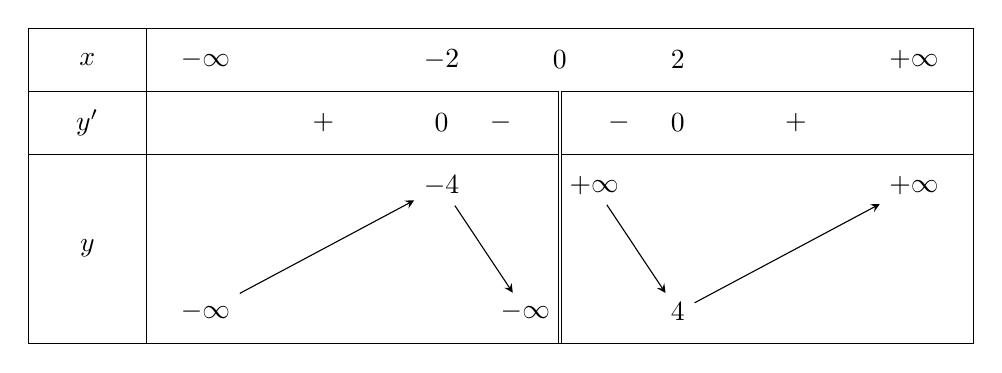
\begin{tikzpicture}[yscale=.8,xscale=1.5,]
					\begin{scope}[shift={(-.5,.5)}]
						\draw
						(0,0) rectangle +(8,-5)
						(0,-1)--+(0:8) (0,-2)--+(0:8) (1,0)--+(-90:5);
					\end{scope}
					\path
					(0,0) node{$x$}          % <<< dòng 1
					++(0:1) node{$-\infty$}
					++(0:2) node{$-2$}
					++(0:1) node{$0$}
					++(0:1) node{$2$}
					++(0:2) node{$+\infty$}
					(0,-1)   node{$y'$}         % <<< dòng 2
					++(0:2) node{$+$}
					++(0:1) node{$0$}
					++(0:.5) node{$-$}
					++(0:1) node{$-$}
					++(0:.5) node{$0$}
					++(0:1) node{$+$}
					(0,-3)   node{$y$}       % <<< dòng 3
					++(0:1) ++(-90:1)  node (A) {$-\infty$}
					++(0:2) ++(90:2) node (B) {$-4$}
					++(0:1) ++(-90:2) node (C)[left]
					{$-\infty$}
					++(90:2) node (D)[right]{$+\infty$}
					++(0:1) ++(-90:2) node (E) {$4$}
					++(0:2) ++(90:2) node (F) {$+\infty$};
					\draw[-stealth] (A)--(B);
					\draw[-stealth] (B)--(C);
					\draw[-stealth] (D)--(E);
					\draw[-stealth] (E)--(F);
					\draw[double] (4,-.5)--(4,-4.5);
				\end{tikzpicture}
			\end{center}
			Hàm số đồng biến trên khoảng $\left( -\infty;-4\right)$ và $\left( 2;+\infty\right)$; nghịch biến trên các khoảng $(-2;0)$ và $(0;2)$.\\
			Hàm số đạt cực đại tại $x=-2$, giá trị cực đại $y=-4$\\
			Hàm số đạt cực tiểu tại $x=2$, giá trị cực tiểu $y=4$
			\item Tập xác định: $\mathscr{D} = \mathbb{R} \setminus \{1\}$.\\
			Đạo hàm: 
			$y' = 1 - \dfrac{9}{(x - 1)^2} = \dfrac{x^2 - 2x - 8}{(x - 1)^2}$.\\
			Cho $y' = 0 \Leftrightarrow x^2 - 2x - 8 = 0 \Leftrightarrow \hoac{& x = -2 \\ & x = 4.}$\\
			Bảng biến thiên:
			\begin{center}
				
\begin{tikzpicture}
					\tkzTabInit[nocadre=false,espcl=2.5,lgt=1.5]
					{$x$/0.6,$y'$/0.6,$y$/2.5}
					{$-\infty$,$-2$,$1$,$4$,$+\infty$}
					\tkzTabLine{,+,0,-,d,-,0,+,}
					\tkzTabVar{-/$-\infty$,+/$-7$,-D+/$-\infty$/$+\infty$,-/$5$,+/$+\infty$}
				\end{tikzpicture}
			\end{center}
		Hàm số đồng biến trên các khoảng $(-\infty; -2)$ và $(4; +\infty)$.\\
		Hàm số nghịch biến trên các khoảng $(-2; 1)$ và $(1; 4)$.\\
		Hàm số đạt cực đại tại $x = -2$, giá trị cực đại $y_{CĐ} = -7$.\\
		Hàm số đạt cực tiểu tại $x = 4$, giá trị cực tiểu $y_{CT} = 5$.
	\end{enumEX}}
\end{vd}
\dongcham{47}

\begin{vd}
	Khảo sát sự biến thiên và tìm cực trị của các hàm số sau:
	\begin{enumEX}[a)]{2}
		\item $y = x \ln x$;
		\item $y = (x^2 - 3)e^x$;
		\item $y = (x^2 - 3)e^{-x}$;
		\item $y = \dfrac{\ln x}{x}$;
		\item $y = \ln(x^2 - 2x + 2)$;
		\item $y = x^2 - 4\ln(1-x)$.
	\end{enumEX}
	\loigiai{
		\begin{enumEX}[a)]{1}
			\item Xét hàm số $y = x \ln x$:
			\begin{itemize}
				\item Tập xác định: $\mathscr{D} = (0; +\infty)$.
				\item Đạo hàm: $y' = \ln x + 1$. Cho $y' = 0 \Leftrightarrow \ln x = -1 \Leftrightarrow x = \dfrac{1}{e}$.
				\item Giới hạn: $\lim\limits_{x \to 0^+} x \ln x = 0$; $\lim\limits_{x \to +\infty} x \ln x = +\infty$.
				\item Bảng biến thiên:
				\begin{center}
					
\begin{tikzpicture}
						\tkzTabInit[nocadre=false,espcl=3,lgt=1.5]
						{$x$/0.6,$y'$/0.6,$y$/2.2}
						{$0$,$\dfrac{1}{e}$,$+\infty$}
						\tkzTabLine{d,-,0,+,}
						\tkzTabVar{D+/$0$,-/$-\dfrac{1}{e}$,+/$+\infty$}
					\end{tikzpicture}
				\end{center}
				\item Kết luận: Hàm số nghịch biến trên $\left(0; \dfrac{1}{e}\right)$, đồng biến trên $\left(\dfrac{1}{e}; +\infty\right)$. Hàm số đạt cực tiểu tại $x = \dfrac{1}{e}$, $y_{CT} = -\dfrac{1}{e}$.
			\end{itemize}
			
			\item Xét hàm số $y = (x^2 - 3)e^x$:
			\begin{itemize}
				\item Tập xác định: $\mathscr{D} = \mathbb{R}$.
				\item Đạo hàm: $y' = (x^2 + 2x - 3)e^x$. Cho $y' = 0 \Leftrightarrow x^2 + 2x - 3 = 0 \Leftrightarrow \hoac{& x = 1 \\ & x = -3.}$
				\item Giới hạn: $\lim\limits_{x \to -\infty} y = 0$; $\lim\limits_{x \to +\infty} y = +\infty$.
				\item Bảng biến thiên:
				\begin{center}
					
\begin{tikzpicture}
						\tkzTabInit[nocadre=false,espcl=2.5,lgt=1.5]
						{$x$/0.6,$y'$/0.6,$y$/2.2}
						{$-\infty$,$-3$,$1$,$+\infty$}
						\tkzTabLine{,+,0,-,0,+,}
						\tkzTabVar{-/$0$,+/$\dfrac{6}{e^3}$,-/$-2e$,+/$+\infty$}
					\end{tikzpicture}
				\end{center}
				\item Kết luận: Hàm số đạt cực đại tại $x = -3$, $y_{CĐ} = \dfrac{6}{e^3}$. Hàm số đạt cực tiểu tại $x = 1$, $y_{CT} = -2e$.
			\end{itemize}
			\item Xét hàm số $y = x^3 e^{-x}$:
			\begin{itemize}
				\item Tập xác định: $\mathscr{D} = \mathbb{R}$.
				\item Đạo hàm: $y' = x^2(3 - x)e^{-x}$. Cho $y' = 0 \Leftrightarrow \hoac{& x = 0 \text{ (nghiệm kép)} \\ & x = 3 \text{ (nghiệm đơn)}.}$
				\item Giới hạn: $\lim\limits_{x \to -\infty} y = -\infty$; $\lim\limits_{x \to +\infty} y = 0$.
				\item Bảng biến thiên:
				\begin{center}
					
\begin{tikzpicture}
						\tkzTabInit[nocadre=false,espcl=2.5,lgt=1.5]
						{$x$/0.6,$y'$/0.6,$y$/2.2}
						{$-\infty$,$0$,$3$,$+\infty$}
						\tkzTabLine{,+,0,+,0,-,}
						\tkzTabVar{-/$-\infty$,R/,+/$\dfrac{27}{e^3}$,-/$0$}
						\tkzTabVal{1}{3}{0.5}{}{$0$}
					\end{tikzpicture}
				\end{center}
				\item Kết luận: Hàm số đồng biến trên $(-\infty; 3)$ và nghịch biến trên $(3; +\infty)$. Hàm số đạt cực đại tại $x = 3$, $y_{CĐ} = \dfrac{27}{e^3}$. Điểm $x=0$ không là điểm cực trị.
			\end{itemize}
			\item Xét hàm số $y = \dfrac{\ln x}{x}$:
			\begin{itemize}
				\item Tập xác định: $\mathscr{D} = (0; +\infty)$.
				\item Đạo hàm: $y' = \dfrac{1 - \ln x}{x^2}$. Cho $y' = 0 \Leftrightarrow 1 - \ln x = 0 \Leftrightarrow x = e$.
				\item Giới hạn: $\lim\limits_{x \to 0^+} y = -\infty$; $\lim\limits_{x \to +\infty} y = 0$.
				\item Bảng biến thiên:
				\begin{center}
					
\begin{tikzpicture}
						\tkzTabInit[nocadre=false,espcl=3,lgt=1.5]
						{$x$/0.6,$y'$/0.6,$y$/2.2}
						{$0$,$e$,$+\infty$}
						\tkzTabLine{d,+,0,-,}
						\tkzTabVar{D-/$-\infty$,+/$\dfrac{1}{e}$,-/$0$}
					\end{tikzpicture}
				\end{center}
				\item Kết luận: Hàm số đạt cực đại tại $x = e$, $y_{CĐ} = \dfrac{1}{e}$. Không có cực tiểu.
			\end{itemize}
			
			\item Xét hàm số $y = x^2 - 4\ln(1 - x)$.
			\begin{itemize}
				\item Điều kiện: $1 - x > 0 \Leftrightarrow x < 1$. 
				Vậy $D = (-\infty; 1)$.
				\item Đạo hàm $y' = 2x - 4 \cdot \dfrac{(1 - x)'}{1 - x} = 2x - 4 \cdot \dfrac{-1}{1 - x} = 2x + \dfrac{4}{1 - x}=\dfrac{-2x^2 + 2x + 4}{1 - x}$.
				\item Bảng biến thiên:
				\begin{center}
					
\begin{tikzpicture}
						\tkzTabInit[nocadre=false,lgt=1.2,espcl=2.5]
						{$x$ /0.6, $y'$ /0.6, $y$ /2}
						{$-\infty$, $-1$, $1$}
						\tkzTabLine{, -, 0, +, d}
						\tkzTabVar{+/$+\infty$, -/$1 - 4\ln 2$, +/$+\infty$}
					\end{tikzpicture}
				\end{center}
				\item Kết luận:
				\begin{itemize}
					\item Hàm số \textbf{nghịch biến} trên khoảng $(-\infty; -1)$.
					\item Hàm số \textbf{đồng biến} trên khoảng $(-1; 1)$.
					\item Hàm số đạt \textbf{cực tiểu} tại $x = -1$, giá trị cực tiểu $y_{\text{CT}} = 1 - 4\ln 2$. Hàm số không có cực đại.
				\end{itemize}
			\end{itemize}
		\end{enumEX}
	}
\end{vd}
\dongcham{35}
\begin{dang}{Bài toán thực tiễn liên quan}
	
\end{dang}

\begin{vd}
	Sau khi một hóa chất bị tràn xuống hồ, nồng độ của hóa chất đó trong nước $C$ (đơn vị: ppm) đo được sau $t$ giờ (kể từ lúc bắt đầu sự cố) tuân theo mô hình:
	$$C(t) = -t^3 + 12t^2 + 60t \quad (0 \le t \le 15)$$
	\begin{enumEX}[a)]{1}
		\item Hãy cho biết nồng độ hóa chất trong hồ tăng hay giảm trong khoảng thời gian từ giờ thứ 12 đến giờ thứ 15?
		\item Sau bao nhiêu giờ kể từ lúc sự cố xảy ra thì nồng độ hóa chất trong hồ đạt mức cao nhất? Mức nồng độ cao nhất đó là bao nhiêu ppm?
	\end{enumEX}
	\loigiai{
		\begin{enumEX}[a)]{1}
			\item Xét hàm số $C(t) = -t^3 + 12t^2 + 60t$ trên đoạn $[0; 15]$.
			Tốc độ thay đổi nồng độ:
			$$C'(t) = -3t^2 + 24t + 60.$$
			Cho $C'(t) = 0 \Leftrightarrow -3(t^2 - 8t - 20) = 0 \Leftrightarrow \hoac{& t = 10 \text{ (thỏa mãn)} \\ & t = -2 \text{ (loại).}}$\\
			Bnagr biến thiên:
			\begin{center}
				
\begin{tikzpicture}
					\tkzTabInit[nocadre=false,espcl=3,lgt=1.5]
					{$t$/0.6,$C'(t)$/0.6,$C(t)$/2.5}
					{$0$,$10$,$15$}
					\tkzTabLine{,+,0,-,}
					\tkzTabVar{-/$0$,+/$800$,-/$225$}
				\end{tikzpicture}
			\end{center}
			Dựa vào bảng biến thiên, trong khoảng thời gian từ giờ thứ 12 đến giờ thứ 15, hàm số $C(t)$ nghịch biến, tức là nồng độ hóa chất trong hồ đang giảm.
			
			\item Dựa vào bảng biến thiên, hàm số đạt giá trị lớn nhất tại $t = 10$.
			Vậy sau $10$ giờ kể từ lúc sự cố xảy ra, nồng độ hóa chất trong hồ đạt mức cao nhất. 
			Mức nồng độ cao nhất là $800$ ppm.
		\end{enumEX}
	}
\end{vd}
\dongcham{13}
\begin{vd} %[Word to LaTeX 3.2]
	Hằng ngày mực nước của hồ thủy điện ở miền Trung lên và xuống theo lượng nước mưa, và các suối nước đổ về hồ. Từ lúc 8h sáng, độ sâu của mực nước trong hồ tính theo mét và lên xuống theo thời gian $t$ (giờ)  cho bởi công thức $h(t)=24t+5t^2-\dfrac{t^3}{3}$. Biết rằng phải thông báo cho các hộ dân phải di dời trước khi xả nước theo quy định trước 5 giờ. Hỏi cần thông báo cho hộ dân di dời lúc mấy giờ trong ngày (tính theo 24 giờ)? Biết rằng mực nước trong hồ phải lên cao nhất mới xả nước.
	\loigiai{
		Ta có $h'(t)=24+10t-t^2$, $h'(t)=0 \Leftrightarrow t=-2$ hoặc $t=12$.\\
		Bảng biến thiên
		\begin{center}
			
\begin{tikzpicture}
				\tkzTabInit[nocadre=false,espcl=2.5,lgt=1.5]
				{$x$/0.6,$h'$/0.6,$h$/1.7}
				{$-\infty$,$-2$,$12$,$+\infty$}
				\tkzTabLine{,-,$0$,+,$0$,-,}
				\tkzTabVar{+/,-/$-\frac{76}{3}$,+/$432$,-/}
			\end{tikzpicture}
		\end{center}
		Nhận xét khi $t=12$ thì mực nước trong hồ lên cao nhất, lúc này thời gian là $8 + 12 = 20$ giờ. Vậy, người ta phải thông báo cho hộ dân di dời lúc $15$ giờ.
		
	}
\end{vd}
\dongcham{11}
\begin{vd}
	Nồng độ $C$ (tính bằng mg/L) của một loại thuốc trong máu bệnh nhân sau khi tiêm $t$ (giờ) được mô hình hóa bởi hàm số:
	$$C(t) = 15t \cdot \mathrm{e}^{-0.2t} \quad (t \ge 0)$$
	\begin{enumEX}[a)]{1}
		\item Lập bảng biến thiên thể hiện sự thay đổi nồng độ thuốc trong máu theo thời gian.
		\item Sau bao lâu kể từ lúc tiêm thì nồng độ thuốc trong máu của bệnh nhân đạt mức cao nhất?
	\end{enumEX}
	\loigiai{
		\begin{enumEX}[a)]{1}
			\item Xét hàm số $C(t) = 15t \cdot \mathrm{e}^{-0.2t}$ trên nửa khoảng $[0; +\infty)$.
			Đạo hàm:
			\begin{align*}
				C'(t) &= (15t)' \cdot \mathrm{e}^{-0.2t} + 15t \cdot \left(\mathrm{e}^{-0.2t}\right)' \\
				&= 15\mathrm{e}^{-0.2t} + 15t \cdot (-0.2)\mathrm{e}^{-0.2t} \\
				&= 15\mathrm{e}^{-0.2t} - 3t\mathrm{e}^{-0.2t} = 3\mathrm{e}^{-0.2t}(5 - t).
			\end{align*}
			Cho $C'(t) = 0 \Leftrightarrow 5 - t = 0 \Leftrightarrow t = 5$ (do $\mathrm{e}^{-0.2t} > 0, \, \forall t$).\\
			Bảng biến thiên:
			\begin{center}
				
\begin{tikzpicture}
					\tkzTabInit[nocadre=false,espcl=3,lgt=1.5]
					{$t$/0.6,$C'(t)$/0.6,$C(t)$/2.5}
					{$0$,$5$,$+\infty$}
					\tkzTabLine{,+,0,-,}
					\tkzTabVar{-/$0$,+/$75\mathrm{e}^{-1}$,-/$0$}
				\end{tikzpicture}
			\end{center}
			
			\item Dựa vào bảng biến thiên, hàm số đồng biến trên khoảng $(0; 5)$ và nghịch biến trên khoảng $(5; +\infty)$. Nồng độ thuốc tăng dần trong $5$ giờ đầu và sau đó giảm dần.\\
			Hàm số đạt giá trị lớn nhất tại $t = 5$. Vậy sau $5$ giờ kể từ lúc tiêm, nồng độ thuốc trong máu của bệnh nhân đạt mức cao nhất (đạt xấp xỉ $27.59$ mg/L).
		\end{enumEX}
	}
\end{vd}
\dongcham{13}
\begin{vd}
	Sau khi một dịch bệnh bùng phát, bộ phận y tế dự phòng ước tính số lượng người nhiễm bệnh $N$ (đơn vị: trăm người) sau $t$ ngày (kể từ lúc phát hiện ca bệnh đầu tiên) được cho bởi hàm số:
	$$N(t) = \dfrac{300t}{t^2 + 9} \quad (t \ge 0)$$
	\begin{enumEX}[a)]{1}
		\item Xét chiều biến thiên của hàm số $N(t)$ để cho biết khoảng thời gian nào số người mắc bệnh tăng, khoảng thời gian nào số người mắc bệnh giảm.
		\item Vào ngày thứ mấy kể từ lúc bùng phát thì số lượng người mắc bệnh là cao nhất? Số lượng cao nhất ước tính là bao nhiêu người?
	\end{enumEX}
	\loigiai{
		\begin{enumEX}[a)]{1}
			\item Xét hàm số $N(t) = \dfrac{300t}{t^2 + 9}$ trên nửa khoảng $[0; +\infty)$.
			Ta có đạo hàm (tốc độ lây lan):
			$$N'(t) = \dfrac{300(t^2 + 9) - 300t \cdot 2t}{(t^2 + 9)^2} = \dfrac{2700 - 300t^2}{(t^2 + 9)^2}.$$
			Cho $N'(t) = 0 \Leftrightarrow 2700 - 300t^2 = 0 \Leftrightarrow t^2 = 9 \Rightarrow t = 3$ (do $t \ge 0$).\\
			Bảng biến thiên:
			\begin{center}
				
\begin{tikzpicture}
					\tkzTabInit[nocadre=false,espcl=3,lgt=1.5]
					{$t$/0.6,$N'(t)$/0.6,$N(t)$/2.5}
					{$0$,$3$,$+\infty$}
					\tkzTabLine{,+,0,-,}
					\tkzTabVar{-/$0$,+/$50$,-/$0$}
				\end{tikzpicture}
			\end{center}
			Kết luận: Hàm số đồng biến trên $(0; 3)$ và nghịch biến trên $(3; +\infty)$.\\
			Điều này có nghĩa là số người nhiễm bệnh tăng liên tục trong 3 ngày đầu tiên và sau đó có xu hướng giảm dần.
			
			\item Dựa vào bảng biến thiên, hàm số $N(t)$ đạt giá trị lớn nhất tại $t = 3$. \\
			Giá trị lớn nhất là $N(3) = 50$ (trăm người).\\
			Vậy vào ngày thứ 3 kể từ lúc bùng phát, số lượng người mắc bệnh là cao nhất. Số lượng ước tính là $50 \times 100 = 5.000$ (người).
		\end{enumEX}
	}
\end{vd}
\dongcham{11}
\boxmini{BÀI TẬP TRẮC NGHIỆM}
\ind{PHẦN I.} \inden{Câu trắc nghiệm nhiều phương án lựa chọn. Mỗi câu hỏi học sinh chỉ chọn một phương án.}\\
\setcounter{ex}{0}
\Opensolutionfile{ans}[ans/2D1-B1-d1-1]

\begin{ex}
	Cho hàm số $y=f(x)$ xác định với mọi $x\ne 4$ và có bảng xét dấu $f'(x)$ như hình vẽ dưới đây. Hàm số đồng biến trên khoảng nào trong các khoảng sau?\\ 
	\begin{center}
\begin{tikzpicture}[scale=0.8]
			\tkzTabInit[nocadre=false,lgt=1.5,espcl=3]
			{$x$ /1,$f'(x)$ /1}
			{$-\infty$,$-1$, $4$, $9$, $+\infty$}
			\tkzTabLine{ ,+,z,-,d,-,z,+, }
		\end{tikzpicture}
		
	\end{center}
	\choice
	{ \True $(-\infty; -1)$ }
	{ $(-2;10)$ }
	{ $(-1; +\infty)$ }
	{ $(-\infty;9)$ }
	\loigiai{ 
		$y'=0 \Leftrightarrow x=-1,x=9$.
		
		Hàm số đồng biến trên các khoảng $(-\infty;-1)$ và $(9;+\infty)$.
		
		Hàm số nghịch biến trên các khoảng $(-1;4)$ và $(4;9)$.
		
		Do đó hàm số đã cho đồng biến trên khoảng $(-\infty; -1)$. 
}\end{ex}

\begin{ex}
	Cho hàm số $y=f(x)$ xác định với mọi $x\ne 4$ và có bảng xét dấu $f'(x)$ như hình vẽ dưới đây. Hàm số nghịch biến trên khoảng nào trong các khoảng sau?\\ 
	\begin{center}
\begin{tikzpicture}[scale=1]
			\tkzTabInit[nocadre=false,lgt=1.5,espcl=3]
			{$x$ /1,$f'(x)$ /1}
			{$-\infty$,$4$,$+\infty$}
			\tkzTabLine{,-, d ,-,}
		\end{tikzpicture}
		
	\end{center}
	\choice
	{ $(0; +\infty)$ }
	{ $(-\infty;+\infty)$ }
	{ \True $(-\infty;2)$ }
	{ $(-\infty;5)$ }
	\loigiai{ 
		Hàm số đã cho nghịch biến trên khoảng $(-\infty;2)$. 
}\end{ex}

\begin{ex}
	\immini[thm]
	{Cho hàm số $y=f(x)$ có đồ thị như hình vẽ bên. Hàm số $y=f(x)$ nghịch biến trên khoảng nào dưới đây?
		\haicot
		{$(\sqrt{2};+\infty)$}
		{$(-2;2)$}
		{$(-\infty;0)$}
		{\True $(0;\sqrt{2})$}
	}
	{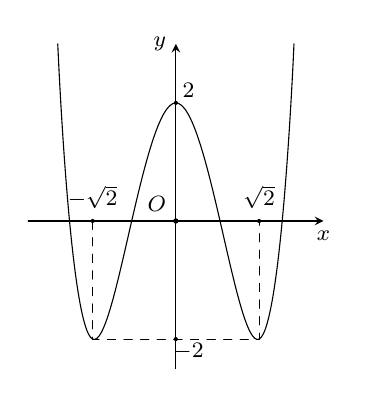
\begin{tikzpicture}[line cap=round,line join=round,x=1.0cm,y=1.0cm,>=stealth,scale=0.75]
			\draw[->,color=black,smooth,samples=100] (-2.5,0.) -- (2.5,0.) node[below] {\footnotesize $x$};
			\draw[->,color=black,smooth,samples=100] (0.,-2.5) -- (0.,3) node[left] {\footnotesize $y$};
			\draw plot[smooth,tension=.7] coordinates {(-2,3) (-1.41,-2)  (0,2) (1.41,-2) (2,3)};
			\draw[fill=black] (0,0) circle [radius=1pt] node[above left] {\footnotesize $O$};
			\fill (-1.41,0) node[shift={(90:2ex)}]{\footnotesize $-\sqrt{2}$} circle(1pt);
			\fill (1.41,0) node[shift={(90:2ex)}]{\footnotesize $\sqrt{2}$} circle(1pt);
			\fill (0,-2) node[shift={(-45:1.5ex)}]{\footnotesize $-2$} circle(1pt);
			\fill (0,2) node[shift={(45:1.5ex)}]{\footnotesize $2$} circle(1pt);
			\draw[dashed] (-1.41,0)|-(0,-2)-|(1.41,0);
	\end{tikzpicture}}
	\loigiai
	{
		Dựa vào đồ thị, ta thấy trên khoảng $(0;\sqrt{2})$ đồ thị đi xuống nên hàm số $y=f(x)$ nghịch biến trên khoảng đó.
	}
\end{ex}

\begin{ex}
	\immini[thm]{Cho hàm số $y=f(x)$ có đồ thị như hình vẽ bên. Mệnh đề nào sau đây là mệnh đề \textbf{sai}?
		\choice
		{Hàm số đạt cực đại tại $x=0$}
		{Hàm số có giá trị cực tiểu bằng $-2$}
		{\True Hàm số đồng biến trên $(-\infty; 2)$}
		{Hàm số nghịch biến trên $(0; 2)$}
	}
	{
		
		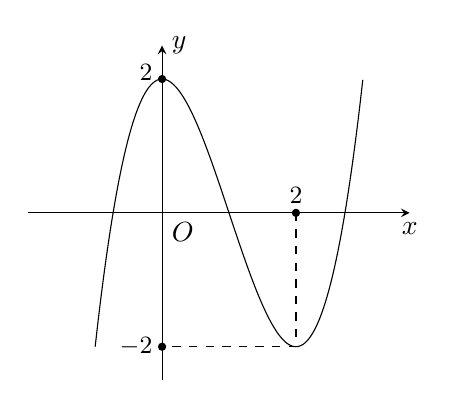
\begin{tikzpicture}[smooth,samples=300,scale=0.85,>=stealth]
			\draw[->] (-2,0)--(3.7,0) node[below]{$x$};
			\draw[->] (0,-2.5)--(0,2.5) node[right]{$y$};
			\draw (0,0) node[below right]{$O$};
			\draw[smooth,samples=100,domain=-1:3]
			plot(\x,{(\x)^3-3*(\x)^2+2});
			\draw[fill=black] (2,0) circle(1.5pt) (0,2) circle(1.5pt) (0,-2) circle(1.5pt);
			\draw[dashed] (2,0)node[above]{\small$2$}--(2,-2)--(0,-2)node[left]{\small$-2$} (0,2.1)node[left]{\small$2$};
		\end{tikzpicture}
	}
	
	\loigiai{
	}
	
\end{ex}

\begin{ex}
	\immini[thm]{
		Hàm số $y=f(x)$ có đồ thị là đường cong trong hình vẽ bên. Hàm số $y=f(x)$ đạt cực tiểu tại điểm nào dưới đây?
		\haicot
		{$x=2$}
		{\True $x=0$}
		{$x=-2$}
		{$x=4$}
	}{
		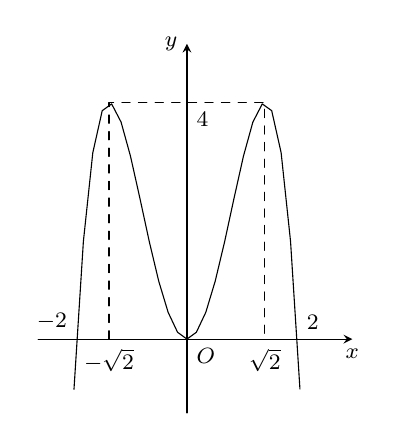
\begin{tikzpicture}[xscale=.7,yscale=.75, font=\footnotesize, line join=round, line cap=round, >=stealth]
			\draw[->] (-2.7,0)--(3,0) node[below]{$x$};
			\draw[->] (0,-1.25)--(0,5) node[left]{$y$};
			\draw[dashed] (-2^.5,0)--(-2^.5,4)--(2^.5,4)--(2^.5,0);
			\draw[domain=-2.05:2.05] plot(\x,{-(\x)^2*((\x)^2-4)});
			\path
			(0,0) node[below right]{$O$}
			(2,0) node[above right]{$2$}
			(-2,0) node[above left]{$-2$}
			(0,4) node[below right]{$4$}
			(-2^.5,0) node[below]{$-\sqrt{2}$}
			(2^.5,0) node[below]{$\sqrt{2}$};
		\end{tikzpicture}
	}
	\loigiai{
		Dựa vào đồ thị hàm số ta thấy hàm số đạt cực tiểu tại $x=0$.}
\end{ex}

\begin{ex}
	\immini[thm]{Cho hàm số $y=f(x)$ có bảng biến thiên như hình bên. Mệnh đề nào sau đây là mệnh đề đúng?
		\choice
		{Hàm số đồng biến trên khoảng $(-\infty;3)$}
		{Hàm số nghịch biến trên khoảng $(-2;+\infty)$}
		{Hàm số đạt cực đại tại $x=3$}
		{\True Hàm số đạt cực tiểu tại $x=2$}}{
		
\begin{tikzpicture}
			\tkzTabInit[lgt=1.2,espcl=2,nocadre=False]
			{$x$/0.7,$f'(x)$/0.7,$f(x)$/2.3}{$-\infty$,$-2$,$2$,$+\infty$}
			\tkzTabLine{,+,0,-,0,+,}
			\tkzTabVar{-/$-\infty$,+/$3$,-/$0$,+/$+\infty$}
	\end{tikzpicture}}
	\loigiai{
	}
	
\end{ex}

\begin{ex}
	\immini[thm]{Cho hàm số $y=f(x)$ có bảng biến thiên bên.	Khẳng định nào sau đây là khẳng định \textbf{sai}?
	\choice
	{Hàm số có hai điểm cực trị}
	{Tọa độ điểm cực đại của đồ thị hàm số là $(-2;-4)$}
	{\True Hàm số nghịch biến trên khoảng $(-2;2)$}
	{Hàm số đồng biến trên khoảng $(3;+\infty)$}
}{

\begin{tikzpicture}
	\tikzset{double style/.append style = {draw=\tkzTabDefaultWritingColor,double=\tkzTabDefaultBackgroundColor,double distance=2pt}}
	\tkzTabInit[lgt=1.2,espcl=1.5,nocadre=False]
	{$x$ /.7, $f’(x)$ /.7,$f(x)$ /2.5}
	{$-\infty$ , $-2$, $0$ ,$2$ ,$+\infty$}
	\tkzTabLine{ ,+,$0$,-,d,-,$0$,+, }
	\tkzTabVar{ -/ $-\infty$,+/ $-4$/,-D+/$- \infty$ /$+\infty$,-/ $4$,+ /$+\infty$}
\end{tikzpicture}}
	\loigiai{
	}
\end{ex}

\begin{ex}
	Gọi $x_1$ là điểm cực đại $x_2$ là điểm cực tiểu của hàm số $y=-x^3+3x+2$. Tính $x_1+2x_2$.
	\choice{$2$}
	{$1$}
	{\True $-1$}
	{$0$}
	\loigiai{
		Ta có $y'=-3x^2+3$, $y'=0\Leftrightarrow x=\pm 1$.\\
		Vì $y'$ đổi dấu từ âm sang dương khi qua $x=-1$ và đổi dấu từ dương sang âm khi qua $x=1$ nên $x_2=-1$ là điểm cực tiểu và $x_1=1$ là điểm cực đại của hàm số. Do đó $x_1+2x_2=1-2=-1$.
	}
\end{ex} \cham{5}


\begin{ex}
	Khoảng cách giữa hai điểm cực trị của đồ thị hàm số $y=x^3-3x^2+4$ bằng
	\choice
	{\True $2\sqrt{5}$}
	{$2\sqrt{2}$}
	{$2$}
	{$ 4 $}
	\loigiai{
		Ta có $y'=3x^2-6x$, $ y'=0\Rightarrow \hoac{&x=0\Rightarrow y=4\\&x=2\Rightarrow y=0.} $\\
		Suy ra hai điểm cực trị của đồ thị hàm số là $A(0;4),B(2;0)$.\\
		Do đó $AB=\sqrt{2^2+(-4)^2}=2\sqrt{5}$.
	}
\end{ex} \cham{6}

\begin{ex}%[2D1B1]
	Hàm số $y=x^4-2x^2+1$ đồng biến trên khoảng nào dưới đây?
	\choice
	{\True $(-1;0)$}
	{$(-1;+ \infty)$}
	{$(-3;8)$}
	{$(- \infty ; -1)$}
	\loigiai
	{
		$y'= 4x^3-4x$ $\Rightarrow y'=0 \Leftrightarrow 4x^3-4x=0$ $\Leftrightarrow \hoac{x&= -1 \\ x&=0 \\ x &= 1}$\\
		Bảng xét dấu
		\begin{center}
			
\begin{tikzpicture}
				\tkzTabInit[nocadre=false, lgt=1, espcl=2.5]{$x$ /1,$y$ /1}{$-\infty$,$-1$,$0$,$1$,$+\infty$}
				\tkzTabLine{,-,$0$,+,$0$,-,$0$,+}
			\end{tikzpicture}
		\end{center}
	}
	
\end{ex} \cham{6}

\begin{ex}%[2HK1-13-ChuyenLeQuyDon-QuangTri]%[2D1B2-1]%
	Cho hàm số $ y = - \dfrac{1}{4}x^4 + \dfrac{1}{2}x^2 - 3 $. Khẳng định nào sau đây là khẳng định đúng?
	\choice
	{Hàm số đạt cực tiểu tại $ x = -3 $}
	{ \True Hàm số đạt cực tiểu tại $ x = 0 $}
	{Hàm số đạt cực đại tại $ x = 0 $}
	{Hàm số đạt cực tiểu tại $ x = -1 $}
	\loigiai{
		Ta có $ y' = - x^3 + x = - x (x^2 - 1) $.
		Ta có bảng biến thiên như hình bên
		\begin{center}
			
\begin{tikzpicture}[scale=1]
				\tkzTabInit[lgt=1.5,espcl=2.5]{$x$  /1,$y'$  /1,$y$ /2}
				{$-\infty$,$ -1 $,$ 0 $,$ 1 $,$+\infty$}%
				\tkzTabLine{,+,z,-,z,+,z,-,}
				\tkzTabVar{-/$ -\infty $,+/   $\dfrac{-11}{4}$ /,-/ $-3$,+/$ \dfrac{-11}{4} $,-/$ -\infty $}
				%\tkzTabIma{1}{3}{2}{$ 0 $}
			\end{tikzpicture}
		\end{center}
	}
\end{ex} \cham{6}

\begin{ex}
	Cho hàm số $y=\dfrac{3x-1}{x-2}$. Mệnh đề nào dưới đây là đúng?
	\choice
	{Hàm số nghịch biến trên $\mathbb{R}$}
	{Hàm số đồng biến trên các khoảng $(-\infty;2)$ và $(2;+\infty)$}
	{\True Hàm số nghịch biến trên các khoảng $(-\infty;2)$ và $(2;+\infty)$}
	{Hàm số đồng biến trên $\mathbb{R}\setminus\{2\}$}
	\loigiai{Tập xác định là $\mathscr{D}=\mathbb{R}\setminus\{2\}$.\\
		Có $y'=\dfrac{-5}{(x-2)^2}<0$, $\forall x\in\mathscr{D}$ nên hàm số nghịch biến trên các khoảng $(-\infty;2)$ và $(2;+\infty)$.}
	
\end{ex} \cham{5}

\begin{ex}
	Cho hàm số $y=\dfrac{x-2}{x+3}$. Mệnh đề nào dưới đây đúng?
	\choice
	{Hàm số nghịch biến trên khoảng $(-\infty;-3)\cup (-3;+\infty) $}
	{\True Hàm số đồng biến trên khoảng $(-\infty;-3) $ và $(-3;+\infty)$}
	{Hàm số nghịch biến trên khoảng $(-\infty;-3)$ và $(-3;+\infty)$}
	{Hàm số đồng biến trên khoảng $(-\infty;-3)\cup (-3;+\infty) $}
	\loigiai{
		Tập xác định $\mathscr{D}=\mathbb{R}\setminus \{-3\}$. Ta có $y'=\dfrac{5}{(x+3)^2}>0$, $\forall x\in\mathscr{D}$.\\ Suy ra hàm số đồng biến trên khoảng $(-\infty;-3)$ và $(-3;+\infty)$.
	}
\end{ex} \cham{6}

\begin{ex}
	Cho hàm số $y=\dfrac{- x^{2} + 4 x - 4}{x - 4}$. Điểm cực tiểu của hàm số đã cho là
	\choice
	{ $x=8$ }
	{ $x=6$ }
	{ $x=-3$ }
	{ \True $x=2$ }
	\loigiai{ 
		
		$y'=- \frac{x^{2} - 8 x + 12}{\left(x - 4\right)^{2}}$.
		
		$y'=0 \Leftrightarrow x=2,x=6$.
		
		Hàm số nghịch biến trên các khoảng $(-\infty;2)$ và $(6;+\infty)$.
		
		Hàm số đồng biến trên các khoảng $(2;4)$ và $(4;6)$.
		
		Do đó đạt cực tiểu tại $x=2$. 
}\end{ex}
\cham{6}
\begin{ex}
	Cho hàm số $y=\dfrac{x^2+3x+3}{x+2}$. Gọi $y_{\text{CĐ}},\,y_{\text{CT}}$ lần lượt là giá trị cực đại và giá trị cực tiểu của hàm số. Giá trị của biểu thức $y_{\text{CĐ}}^2-2y_{\text{CT}}^2$ bằng
	\choice
	{$8$}
	{\True $7$}
	{$9$}
	{$6$}
	\loigiai{
		Ta có $y'=\dfrac{x^2+4x+3}{(x+2)^2}$; $y'=0 \Leftrightarrow \left[\begin{aligned}
			&x=-1 \\
			&x=-3
		\end{aligned}\right. $. \\
		Bảng biến thiên
		\begin{center}
			
\begin{tikzpicture}
				\tkzTab
				[lgt=1,espcl=2] % tùy chọn
				{$x$/0.7, $y'$/0.7, $y$/2} % cột đầu tiên
				{$-\infty$, $-3$, $-2$, $-1$, $+\infty$} % hàng 1 cột 2
				{,+,0,-,d,-,0,+,} % hàng 2 cột 2
				{-/ $-\infty$, +/ $-3$, -D+/ $-\infty$ / $+\infty$, -/ $1$, +/ $+\infty$} % hàng 3 cột 2
			\end{tikzpicture}
		\end{center}
		Từ bảng biến thiên ta tìm được $y_{\text{CĐ}}=-3;\,y_{\text{CT}}=1$ $ \Rightarrow $ $y_{\text{CĐ}}^2-2y_{\text{CT}}^2$ $=9-2=7$.}
\end{ex} \cham{6}

\begin{ex}
	Tìm điểm cực tiểu của hàm số $f(x)=(x-3)\mathrm{e}^x$.
	\choice
	{$x=3$}
	{$x=0$}
	{\True $x=2$}
	{$x=1$}
	\loigiai{
		\begin{itemize}
			\item Ta có $f'(x)=\mathrm{e}^x(x-2)$, $f''(x)=\mathrm{e}^x(x-1)$.
			\item $f'(x)=0\Rightarrow x=2$ và $f''(2)=\mathrm{e}^2>0$.
		\end{itemize}
		Vậy hàm số đã cho đạt cực tiểu tại $x=2$.}
\end{ex} \cham{8}

\begin{ex}
	Cho hàm số $y=x^2+4\ln(3-x)$. Tìm giá trị cực đai $y_\text{CĐ}$ của hàm số đã cho.
	\choice
	{$y_\text{CĐ}=2$}
	{\True $y_\text{CĐ}=4$}
	{$y_\text{CĐ}=1+4\ln2$}
	{$y_\text{CĐ}=1$}
	\loigiai{
		Tập xác định $\mathscr{D}=(-\infty;3)$.\\
		Đạo hàm $y'=2x-\dfrac{4}{3-x}=\dfrac{-2x^2+6x-4}{3-x}$.\\
		$y'=0\Leftrightarrow -2x^2+6x-4=0\Leftrightarrow \hoac{&x=1\\&x=2}$.\\
		Bảng biến thiên
		\begin{center}
			
\begin{tikzpicture}[>=stealth]
				\tkzTabInit[nocadre=false,lgt=1,espcl=2,deltacl=0.5]{$x$/.7,$y'$/.7,$y$/2}
				{$-\infty$,$1$,$2$,$3$}
				\tkzTabLine{,-,0,+,0,-,d}
				\tkzTabVar{+/$+\infty$,-/$1+4\ln 2$,+/$4$,-D/$-\infty$}
			\end{tikzpicture}
		\end{center}
		Hàm số đạt cực đại tại $x=2$, $y_\text{CĐ}=4$.
	}
\end{ex} \cham{8}

\begin{ex}%[2D1B2]
	Cho hàm số $ y=f(x) $ liên tục trên $ \mathbb{R} $ và có đạo hàm $ f'(x)=x(x-1)^2(x-2)^3 $. Số điểm cực trị của hàm số $ y=f(x) $ là
	\choice{1}{\True 2}{0}{3}
	\loigiai{	Ta có bảng xét dấu của $ f'(x) $:
		\begin{center}
			
\begin{tikzpicture}
				\tkzTabInit[lgt=2,espcl=1.5]%
				{$x$ /1,$f'(x)$ /1}
				{$-\infty$ , $0$ , $1$ , $2$ ,$+\infty$}
				\tkzTabLine{ ,+,0,-,0,-,0,+,}
			\end{tikzpicture}
		\end{center}
		Dựa vào bảng xét dấu ta thấy $ f(x) $ có 2 điểm cực trị.
}\end{ex} \cham{7}



\begin{ex}%[2D1K2-2]%
	\immini[thm]{Cho hàm số bậc bốn $ y=f(x) $. Biết $f'(x) $ có đồ thị như hình bên. Khẳng định nào sau đây là khẳng định đúng?
		\choice
		{Hàm số $f(x)$ đồng biến trên khoảng $(-\infty;0)$}
		{Hàm số $f(x)$ nghịch biến trên khoảng $(-1;1)$}
		{Hàm số $f(x)$ có đúng một điểm cực tiểu}
		{\True Hàm số $f(x)$ có đúng một điểm cực đại}
	}{
		\begin{tikzpicture}[>=stealth,line join=round,line cap=round,font=\footnotesize,scale=0.7,smooth]
			\draw[->] (-3,0)--(7,0)node[below]{$x$};
			\foreach \x in {-2,-1,1,2,3,4}\draw[shift={(\x,0)}] (0,2pt)--(0,-2pt) node[below]{\scriptsize $\x$};
			\draw[->] (0,-2)--(0,3)node[right]{$y$};
			\draw[] plot[smooth,tension=.65] coordinates{(-1.7,-2) (-1,0) (0,.7) (1,0)(2.7,-1.2)(4,0) (5,2.5)}node[right]{$y=f'(x)$};
		\end{tikzpicture}
	}
	\loigiai{
		\immini{Dựa vào đồ thị, ta có bảng biến thiên như hình vẽ. \\
		}{% Cần khai báo \usepackage{tkz-tab}
			
\begin{tikzpicture}[scale=.8, font=\footnotesize, line join=round, line cap=round, >=stealth]
				\tkzTabInit[nocadre=false,lgt=1,espcl=2,deltacl=0.5]{$x$/.7 ,$y'$/.7,$y$/2}
				{$-\infty$ , $-1$ , $1$, $ 4 $, $+\infty$}
				\tkzTabLine{ , - , $0$ ,+, $ 0 $, -, $0$ , + , }
				\tkzTabVar{+/$+\infty$ , -/$f(-1)$ ,+/$f(-1)$ ,-/$ f(4) $, +/$+\infty$}
		\end{tikzpicture}}
	}
\end{ex} \cham{7}

\begin{ex}
	\immini[thm]{
		Cho hàm số $y=f(x)$ xác định và liên tục trên $\mathbb{R}$. Biết rằng hàm số $f(x)$ có đạo hàm $f'(x)$ và hàm số $y=f'(x)$ có đồ thị như hình vẽ. Khi đó nhận xét nào sau đây đúng?
		\choice
		{\True Hàm số $f(x)$ không có cực trị}
		{Đồ thị hàm số $f(x)$ có đúng $2$ điểm cực tiểu}
		{Đồ thị hàm số $f(x)$ có đúng một cực đại}
		{Hàm số $f(x)$ có $3$ cực trị}
	}{
		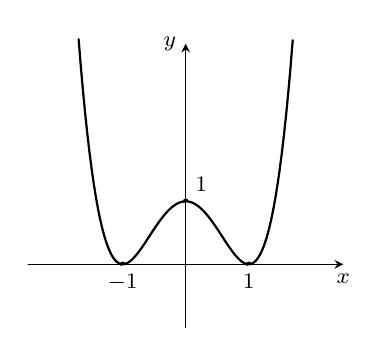
\begin{tikzpicture}[scale=.8,font=\footnotesize, line join=round,line cap=round,>=stealth]
			\draw[->] (-2.5,0)--(2.5,0)node[below]{$x$};
			\draw[->] (0,-1)--(0,3.5)node[left]{$y$};
			\draw[thick,samples=100,domain=-1.7:1.7] plot(\x,{(\x)^4-2*(\x)^2+1});
			\draw[dashed] (-1,0)node[below]{$-1$}circle(1pt) (1,0)node[below]{$1$}circle(1pt) (0,1)node[above right]{$1$}circle(1pt);
		\end{tikzpicture}
	}
	\loigiai{
		Dựa vào đồ thị ta thấy $f'(x)\geq 0$, với mọi $x\in\mathbb{R}$.\\
		Suy ra, hàm số $f(x)$ không có cực trị.
	}
\end{ex} \cham{8}


\Closesolutionfile{ans}

\ind{PHẦN II.} \inden{Câu trắc nghiệm đúng sai. Trong mỗi ý a), b), c), d) ở mỗi câu, học sinh chọn đúng hoặc sai.}\\
\Opensolutionfile{ans}[ans/2D1-B1-d1-2]

\begin{ex}
	Cho hàm số $y=f(x)$ liên tục trên $\mathbb{R}$ và có bảng xét dấu đạo hàm như hình bên.
	\immini{
		\choiceTF
		{Hàm số đồng biến trên khoảng $(-\infty;1)$}
		{\True Hàm số đồng biến trên khoảng $(1;+\infty)$}
		{Hàm số đạt cực đại tại $x=2$}
		{Hàm số có một điểm cực đại và hai điểm cực tiểu}
	}{\vspace{0.1cm}
		
\begin{tikzpicture}
			\tikzset{double style/.append style = {draw=\tkzTabDefaultWritingColor,double=\tkzTabDefaultBackgroundColor,double distance=2pt}}
			\tkzTabInit[nocadre=false, lgt=1, espcl=1.2]{$x$ /0.7,$y'$ /1}{$-\infty$,$0$,$1$,$2$,$+\infty$}
			\tkzTabLine{,+,$0$,-,d,+,$0$,+,}
		\end{tikzpicture}}
	\loigiai{
		Ta có bảng biến thiên như sau:
		\begin{center}
			
\begin{tikzpicture}
				\tikzset{double style/.append style = {draw=\tkzTabDefaultWritingColor,double=\tkzTabDefaultBackgroundColor,double distance=2pt}}
				\tkzTabInit[lgt=1.1,espcl=2,nocadre=True]
				{$x$ /.7, $y'$ /.7,$y$ /2}
				{$-\infty$ , $0$, $1$ ,$2$ ,$+\infty$}
				\tkzTabLine{ ,+,$0$,-,d,+,$0$,+, }
				\tkzTabVar{ -/,+/ /,-/,R,+/$+\infty$}
			\end{tikzpicture}
		\end{center}
	Từ đây, suy ra:
		\begin{enumerate}[a)]
			\item Hàm số đồng biến trên khoảng $(-\infty;1)$ là khẳng định sai.
			\item Hàm số đồng biến trên khoảng $(1;+\infty)$ là khẳng định đúng.
			\item Hàm số đạt cực đại tại $x=2$ là khẳng định sai.
			\item Hàm số có một điểm cực đại và hai điểm cực tiểu là khẳng định sai.
		\end{enumerate}
	}
	
\end{ex} \cham{4}

\begin{ex}
	Cho hàm số $y=x^3-3x^2+4$ có đồ thị $(C)$. Gọi $A$, $B$ là hai điểm cực trị của $(C)$.
	\choiceTF
	{\True Tập xác định của hàm số là $\mathbb{R}$}
	{Hàm số đồng biến trên khoảng $(0;2)$}
	{\True Phương trình đường thẳng qua hai điểm cực trị của đồ thị hàm số là $2x+y-4=0$}
	{\True Diện tích của tam giác $OAB$ bằng $4$, với $O$ là gốc tọa độ}
	\loigiai{
		\begin{enumerate}[a)]
			\item Hàm số đa thức nên có tập xác định là $D=\mathbb{R}$.
			\item Ta có 
			\begin{itemize}
				\item [$\bullet$] $y'=3x^2-6x$ và $y'=0 \Leftrightarrow x=0$ hoặc $x=2$.
			\end{itemize}
			Bảng biến thiên:
			\begin{center}
				
\begin{tikzpicture}
					\tkzTabInit[lgt=1,espcl=3]
					{$x$ /0.7, $y'$ /0.7, $y$ /2.5}
					{$-\infty$,$0$,$2$,$+\infty$}
					\tkzTabLine{,+,$0$,-,$0$,+,}
					\tkzTabVar{-/$-\infty$,+/$4$,-/$0$,+/$+\infty$}
				\end{tikzpicture}
			\end{center}
		Suy ra hàm nghịch biến trên $(0;2)$.
			\item Tọa độ $A(0;4)$, $B(2;0)$. Phương trình đường thẳng $AB$ là
			$$\dfrac{x-0}{2-0}=\dfrac{y-4}{0-4} \Leftrightarrow 2x+y-4=0$$
			\item Diện tích tam giác vuông $OAB$ là $S_{OAB}=\dfrac{1}{2}OA \cdot OB=4$.
		\end{enumerate}

	}
\end{ex} \cham{9}

\begin{ex}
	Cho hàm số $y=\dfrac{x^2+2x+2}{x+1}$ có đồ thị $(C)$. Gọi $A$, $B$ lần lượt là điểm cực tiểu và điểm cực đại của $(C)$.
	\choiceTF
	{Tập xác định của hàm số là $\mathbb{R}$}
	{Hàm số nghịch biến trên khoảng $(-2;0)$}
	{Tọa độ điểm $A(-2;-2)$, $B(0;2)$}
	{\True Khoảng cách giữa hai điểm cực trị là $AB=2\sqrt{5}$}
	\loigiai{
		\begin{enumerate}[a)]
			\item Đặt điều kiện mẫu số khác 0, ta được $x+1 \ne 0 \Leftrightarrow x \ne -1$. Suy ra $\mathscr{D}=\mathbb{R}\setminus \left\{-1\right\}$.
			\item $y'=\dfrac{x^2+2x}{(x+1)^2}\Rightarrow y'=0\Leftrightarrow \hoac{& x=-2 \\ & x=0.}$\\
			Ta có bảng xét dấu của hàm $f'(x)$ như sau
			\begin{center}
					
\begin{tikzpicture}
					\tkzTabInit[nocadre=false,lgt=1,espcl=3]
					{$x$ /0.7,$y'$ /0.7,$y$ /2}
					{$-\infty$,$-2$,$-1$,$0$,$+\infty$}
					\tkzTabLine{,+,$0$,-,d,-,$0$,+,}
					\tkzTabVar{-/$-\infty$,+/$-2$,-D+/$-\infty$/$+\infty$,-/$2$,+/$+\infty$}
				\end{tikzpicture}
			\end{center}
			Dựa vào bảng xét dấu ta thấy rằng hàm số $y=f'(x)$ nghịch biến trên $(-2;-1)$ và $(-1;0)$.
			\item Tọa độ điểm $A(0;2)$, $B(-2;-2)$
			\item Độ dài $AB=\sqrt{(-2-0)^2+(-2-2)^2}=2\sqrt{5}$.
		\end{enumerate}

	}
\end{ex} \cham{8}


\begin{ex}
	Xét một chất điểm chuyển động dọc theo trục $Ox$. Toạ độ của chất điểm tại thời điểm $t$ được xác định bởi hàm số $x(t)=t^3-6t^2+9t$ với $t\geq 0$. Khi đó $x'(t)$ là vận tốc của chất điểm tại thời điểm $t$, kí hiệu $v(t)$; $v'(t)$ là gia tốc chuyển động của chất điểm tại thời điểm $t$, kí hiệu $a(t)$.
	\choiceTF
	{Phương trình hàm vận tốc là $v(t)=3t^2-6t+9$}
	{\True Phương trình hàm gia tốc là $a(t)=6t-12$}
	{Vận tốc của chất điểm tăng khi $t\in (0;1)$ hoặc  $t \in (3;+\infty)$}
	{Vận tốc của chất điểm giảm khi $t\in (1;3)$}
	\loigiai{
		\begin{enumerate}
			\item $v(t)=x'(t)=3t^2-12t+9$
			\item $a(t)=v'(t)=6t-12$.
			\item Xét $v'(t)=6t-12$, $v'(t)=0\Leftrightarrow t=2$\\
			Bảng xét dấu
			\begin{center}
				
\begin{tikzpicture}
					\tkzTabInit[nocadre=false,lgt=2,espcl=2.1]
					{$t$ /0.6,$v'(t)$ /0.6}
					{$0$,$2$,$+\infty$}
					\tkzTabLine{,-,$0$,+,}
				\end{tikzpicture}
			\end{center}
			Suy ra vận tốc của chất điểm tăng khi $t\in (2;+\infty) $, giảm khi $t\in (0;2)$.
		\end{enumerate}
	}
\end{ex} \cham{10}

\Closesolutionfile{ans}
\ind{PHẦN III.} \inden{Câu trắc nghiệm trả lời ngắn. Thí sinh trả lời các câu hỏi sau vào ô kết quả.}\\
\Opensolutionfile{ans}[ans/2D1-B1-d1-3]
\begin{ex}
	Cho hàm số $y=f(x)=- \dfrac{x^{3}}{3} + \dfrac{x^{2}}{2} + 2 x - 2$ có giá trị cực tiểu bằng $y_1$ và giá trị cực đại bằng $y_2$. Tính $P=4y_1+4y_2$ (\textit{kết quả làm tròn đến hàng phần mười}).\\ 
	\shortans[oly]{$-7,3$}
	\loigiai{ 
		$f'(x)=- x^{2} + x + 2$.
		
		$f'(x)=0 \Leftrightarrow x=-1$ hoặc $x=2$.
		
		Lập bảng biến thiên.
		
		Hàm số đạt cực tiểu tại $x_1=-1$, đạt cực đại tại $x_2=2$.
		
		$y_1=f(-1)=- \frac{19}{6}, y_2=f(2)=\frac{4}{3}$.
		
		$P=4y_1+4y_2=- \frac{22}{3}$.
		
		Đáp án: $-7,3 $ 
}\end{ex}
\cham{6}
\begin{ex}
	Cho hàm số $y=f(x)=\dfrac{2 x^{2} + 12 x + 8}{x + 6}$ có giá trị cực tiểu bằng $y_1$ và giá trị cực đại bằng $y_2$. Tính $P=- y_{1} + 2 y_{2}$ (\textit{kết quả làm tròn đến hàng phần mười}).\\ 
	\shortans[oly]{$-36,0$}
	
	\loigiai{ 
		$f'(x)=\frac{2 \left(x^{2} + 12 x + 32\right)}{\left(x + 6\right)^{2}}$.
		
		$f'(x)=0 \Leftrightarrow x=-8$ hoặc $x=-4$.
		
		Lập bảng biến thiên.
		
		Hàm số đạt cực tiểu tại $x_1=-4$, đạt cực đại tại $x_2=-8$.
		
		$y_1=f(-4)=-4, y_2=f(-8)=-20$.
		
		$P=- y_{1} + 2 y_{2}=-36$. 
}\end{ex}
\cham{6}

\begin{ex}
	Chỉ số ô nhiễm bụi mịn PM2.5 tại một thành phố trong những tuần đầu năm được đo đạc và xấp xỉ bằng hàm số $I(t) = -2t^3 + 33t^2 + 72t + 50$, trong đó $t$ là số tuần lễ tính từ đầu năm ($t \ge 0$). Sau bao nhiêu tuần lễ kể từ đầu năm thì chỉ số ô nhiễm tại thành phố này đạt mức cao nhất? \\
	\shortans[oly]{$12$}
	\loigiai{
		Xét hàm số $I(t) = -2t^3 + 33t^2 + 72t + 50$ trên nửa khoảng $[0; +\infty)$.
		Ta có đạo hàm: $I'(t) = -6t^2 + 66t + 72$. \\
		Cho $I'(t) = 0 \Leftrightarrow -6(t^2 - 11t - 12) = 0 \Leftrightarrow \hoac{& t = 12 \text{ (thỏa mãn)} \\ & t = -1 \text{ (loại).}}$
		Bảng biến thiên:
		\begin{center}
			
\begin{tikzpicture}
				\tkzTabInit[nocadre=false,espcl=3,lgt=1.5]
				{$t$/0.6,$I'(t)$/0.6,$I(t)$/2.5}
				{$0$,$12$,$+\infty$}
				\tkzTabLine{,+,0,-,}
				\tkzTabVar{-/$50$,+/$2210$,-/$-\infty$}
			\end{tikzpicture}
		\end{center}
		Dựa vào bảng biến thiên, hàm số đạt giá trị lớn nhất tại $t = 12$.
		Vậy sau $12$ tuần lễ, chỉ số ô nhiễm đạt mức cao nhất.
	}
\end{ex}
\cham{7}
\begin{ex}
	Khi loại thuốc A được tiêm vào bệnh nhân, nồng độ mg/l của thuốc trong máu sau $x$ phút (kể từ khi bắt đầu tiêm) được xác định bởi công thức $C(x)=\dfrac{30 x}{x^2+2}$. Để đưa ra những lời khuyên và cách xử lí phù hợp cho bệnh nhân, ta cần tìm khoảng thời gian mà nồng độ của thuốc trong máu đang tăng. Hãy cho biết hàm nồng độ thuốc trong máu $C(x)$ đạt giá trị cực đại là bao nhiêu trong khoảng thời gian 6 phút sau khi tiêm (\textit{kết quả làm tròn đến hàng phần mười})?\\
	\shortans[oly]{$10,6$}
	\loigiai{
		Xét hàm số $y=C(x)=\dfrac{30 x}{x^2+2}$ trên khoảng $x \in(0 ; 6)$.\\
		Ta có: $y^{\prime}=\dfrac{-30 x^2+60}{\left(x^2+2\right)^2}$.$$
		y^{\prime}=0 \Leftrightarrow \dfrac{-30 x^2+60}{\left(x^2+2\right)^2}=0 \Leftrightarrow\left[\begin{array}{l}
			x=\sqrt{2} \\
			x=-\sqrt{2}
		\end{array} \text { do } x \in(0 ; 6) \Rightarrow x=\sqrt{2} .\right.
		$$
		Bảng biến thiên:
		\begin{center}
			
\begin{tikzpicture}
				\tkzTabInit[nocadre=false,lgt=1.2,espcl=4,deltacl=0.6]
				{$x$/0.6, $y’$/0.6,$y$/2}
				{$0$,$\sqrt{2}$,$6$}
				\tkzTabLine{,+,$0$,-}
				\tkzTabVar{-/$0$,+/$\frac{15\sqrt{2}}{2}$,-/$\frac{90}{19}$}
			\end{tikzpicture}	
		\end{center}
		Suy ra, $C(x)$ đạt giá trị cực đại là $\dfrac{15\sqrt{2}}{2}\approx 10,6$.
	}
\end{ex}
\cham{7}
\begin{ex}%[2D1H1-5]
	Sự ảnh hưởng khi sử dụng một loại độc tố với vi khuẩn $X$ được một nhà sinh học mô tả bởi hàm số $P(t)=\dfrac{t+1}{t^2+t+4}$, trong đó $P(t)$ là số lượng vi khuẩn sau $t$ giờ sử dụng độc tố. Vào thời điểm nào thì số lượng vi khuẩn $X$ bắt đầu giảm? \\
	\shortans[oly]{$1$}
	\loigiai{
		Ta có $P'(t)=\dfrac{-t^2-2t+3}{\left(t^2+t+4\right)^2}=\dfrac{(t-1)(-t-3)}{\left(t^2+t+4\right)^2} \quad (t>0)$.\\
		$\Rightarrow 	P'(t)=0 \Leftrightarrow \hoac{&t=-3 \quad \text{(loại)}\\&t=1 \quad \text{(nhận)}.}$\\
		Bảng biến thiên 
		\begin{center}
			
\begin{tikzpicture}[scale=1, font=\footnotesize, line join=round, line cap=round, >=stealth]
				\tkzTabInit[nocadre=false,lgt=1.5,espcl=2,deltacl=0.5]
				{$t$/.7 ,$P'(t)$/.7,$P(t)$/2}
				{$0$ , $1$ , $+\infty$}
				\tkzTabLine{ , + , $0$ , - , }
				\tkzTabVar{-/$\dfrac{1}{4}$ , +/$\dfrac{1}{3}$ , -/$0$}
			\end{tikzpicture}
		\end{center}
		Ta thấy hàm số đạt cực đại tại $t=1$ và $P'(t)<0, \forall t \in(1;+\infty)$ nên sau $1$ giờ thì vi khuẩn bắt đầu giảm.
	}
\end{ex}
\cham{7}
\begin{ex}
	\immini[thm]{
		Máng trượt của một cầu trượt cho trẻ em được uốn từ một tấm kim loại có bề rộng $80$ cm, mặt cắt được mô tả ở hình bên. Nhà thiết kế khuyến cáo, diện tích mặt cắt càng lớn thì càng đảm bảo an toàn cho trẻ em. Với $x$ đạt giá trị bằng bao nhiêu thì cầu trượt đảm bảo an toàn nhất cho trẻ em?
		\\
		\shortans[oly]{$20$}
	}{
		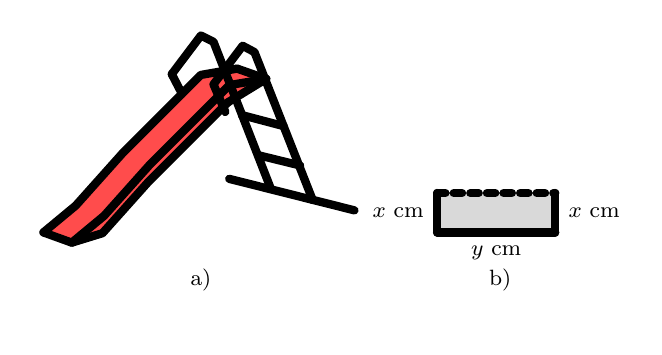
\begin{tikzpicture}[scale=1, font=\footnotesize, line join=round, line cap=round, >=stealth,line width=3.pt]
			\clip(-0.2,-1.2) rectangle (7.5,2.6);
			\fill[line width=3.pt,color=red,fill=red,fill opacity=0.7] (0,0)--(0.41,0.34)--(1,1)--(1.76,1.76)--(2,2)--(2.46,2.08)--(2.83,1.95)--(2.34,1.65)--(1.34,0.65)--(0.75,-0.01)--(0.36,-0.13)-- cycle;
			\draw (0,0)--(0.41,0.34)--(1,1)--(2,2)--(2.46,2.08);
			\draw (0,0)--(0.36,-0.13)--(0.77,0.21)--(0.77,0.21)--(1.36,0.87)--(2.36,1.87)--(2.83,1.95);
			\draw (0.36,-0.13)--(0.75,-0.01)--(1.34,0.65)--(2.34,1.65);
			\draw (2.36,0.68)-- (3.95,0.28);
			\draw (3.42,0.41)--(2.68,2.29)--(2.53,2.37)--(2.16,1.88)--(2.31,1.53);
			\draw (1.63,2.01)--(2,2.5)-- (2.16,2.42)--(2.89,0.55);
			\draw (1.63,2.01)--(1.76,1.76) (2.73,0.98)--(3.26,0.85) (2.52,1.49)--(3.05,1.35);
			\draw (2.34,1.65)--(2.83,1.95)--(2.46,2.08);
			\draw (2,-0.6)node{a)};
			\fill[line width=3.pt,fill=gray,fill opacity=0.3] (5,0.5)--(5,0)--(6.5,0)--(6.5,0.5)--cycle;
			\draw (5,0.5)--(5,0) node [left ,sloped,pos=0.5,rotate=90] {$x$ cm};
			\draw (5,0)--(6.5,0) node [below,sloped,pos=0.5] {$y$ cm};
			\draw (6.5,0)--(6.5,0.5) node [right,sloped,pos=0.5,rotate=-90] {$x$ cm};
			\draw[dashed] (5,0.5)--(6.5,0.5);
			\draw (5.8,-0.6)node{b)};
			\end{tikzpicture}
	}
	\loigiai{
		\begin{enumerate}[$\bullet$]
			\item Do tấm kim loại có bề rộng $80 \mathrm{~cm}$ nên ta có: $2x+y=80 \Leftrightarrow y=80-2x$.\\
			Để có thể thiết kế được máng trượt thì $y>0 \Leftrightarrow 80-2 x>0 \Leftrightarrow x<40$. Suy ra $0<x<40$.\\
			Diện tích của mặt cắt máng trượt là: $S=x y=x(80-2x)=-2x^2+80x$.		
			\item Ta có: 
			\allowdisplaybreaks
			\begin{eqnarray*}
				S(x)&=&-2x^2+80x \text{ với } x\in(0; 40);\\
				S'(x)&=&-4 x+80 \\
				S'(x)&=&0 \Leftrightarrow-4 x+80=0 \Leftrightarrow x=20.
			\end{eqnarray*}
			Bảng biến thiên của hàm số $S(x)$ như sau:
			\begin{center}
				
\begin{tikzpicture}[font=\footnotesize,thick,>=stealth]
					\tikzset{double style/.append style={double distance=1.5pt}}
					\tkzTabInit[nocadre=false,lgt=1.2,espcl=2.5,deltacl=0.6,lw=.75pt,color,colorL=green!50,colorV=green!50]
					{$x$ /0.7, $S'(x)$ /0.8, $S(x)$ /2}
					{$0$,$20$,$40$}
					\tkzTabLine{ ,+,,-, }
					\tkzTabVar{-/$0$,+/$800$,-/$0$}
				\end{tikzpicture}
			\end{center}
			Do đó, hàm số $S(x)$ đạt cực đại tại $x=20$ và $S_{\text{CĐ}}=800$.\\
			Vậy để cầu trượt đảm bảo an toàn nhất cho trẻ em thì $x=20$ (cm).
		\end{enumerate}
	}
\end{ex}
\cham{12}

\Closesolutionfile{ans}